\section{系统问题总结}
\subsection{关于系统软关机复位问题}
Q:系统软关机使用内置触摸和普通IO关机,开机时\emphasizebox{reset}位置有什么不同?
\begin{itemize}
    \item 普通IO关机,P11系统会掉电,指剩下P33维持电压,开机\emphasizebox{reset}是从\emphasizebox{maskrom}的\emphasizebox{startup}开始;
    \item 使用内置触摸关机,P11系统维持电源工作,这是关机之后还会大几\emphasizebox{uA}的原因,开机\emphasizebox{reset}也是从\emphasizebox{maskrom}的\emphasizebox{Startup}开始;
\end{itemize}

\subsection{关于使用内置触摸开机ROM中IO状态恢复出错问题}
Q:当使用内置触摸开机时,发现\emphasizebox{PC3 IO}变为输出低状态,关机之前在mask\_IO中已经把IO状态设置为高阻?
\begin{itemize}
    \item 当使用\emphasizebox{LPCTMU}关机时,会使用\emphasizebox{PLCNT}模块,配置了\emphasizebox{P3\_PCNT\_SET0}和\emphasizebox{P3\_PCNT\_SET1}两个寄存器,\emphasizebox{PC3 IO}状态正好配置了3,导致在mask恢复IO时设置为输出0状态;
    \item 解决办法:在\emphasizebox{soft\_off\_enter}和\emphasizebox{soft\_off\_exit}时加入\emphasizebox{save}和\emphasizebox{recover}流程即可。
\end{itemize}

\subsection{br28 ass ASS\_CLK\_CON bit7写完和读出来不一样问题(bit5)}
问题:在写ASS\_CLK\_CON的bit7置1时,写完读出来是0x40,再写bit7置0时,读出来时0x20;

解释:由于bit5没有用到,cpu读会移位,在软件层面第一次写bit7置1时,cpu行为:
\begin{myccode}
    {
        int bak = 0;
        bak = ASS_CLK_CON;
        bak |= BIT(7);
        ASS_CLK_CON = bak;
    }
\end{myccode}
由于bit5没用到,在cpu读时,bit6变bit5,bit7变bit6,因此写完bit7之后,读出来是0b0100,0000 = 0x40,再把bit7写0时,cpu行为:
\begin{myccode}
    {
        int bak = 0;
        bak = ASS_CLK_CON;  //此时bak = 0b0100,0000
        bak &= ~BIT(7);     //此时bak = 0b0100,0000
        ASS_CLK_CON = bak;  //写bit7为0无效;
    }
\end{myccode}
下次再写bit7,将会读回来是0b1100, 0000 = 0xC0,导致出错,硬件Bug;

\subsection{br34 RVDD电压要大于等于DVDD问题}
如果RVDD < DVDD时,有的板子会出现程序跑到某个ram地址出现非对齐访问异常问题。
\begin{figure}[H]
\centering
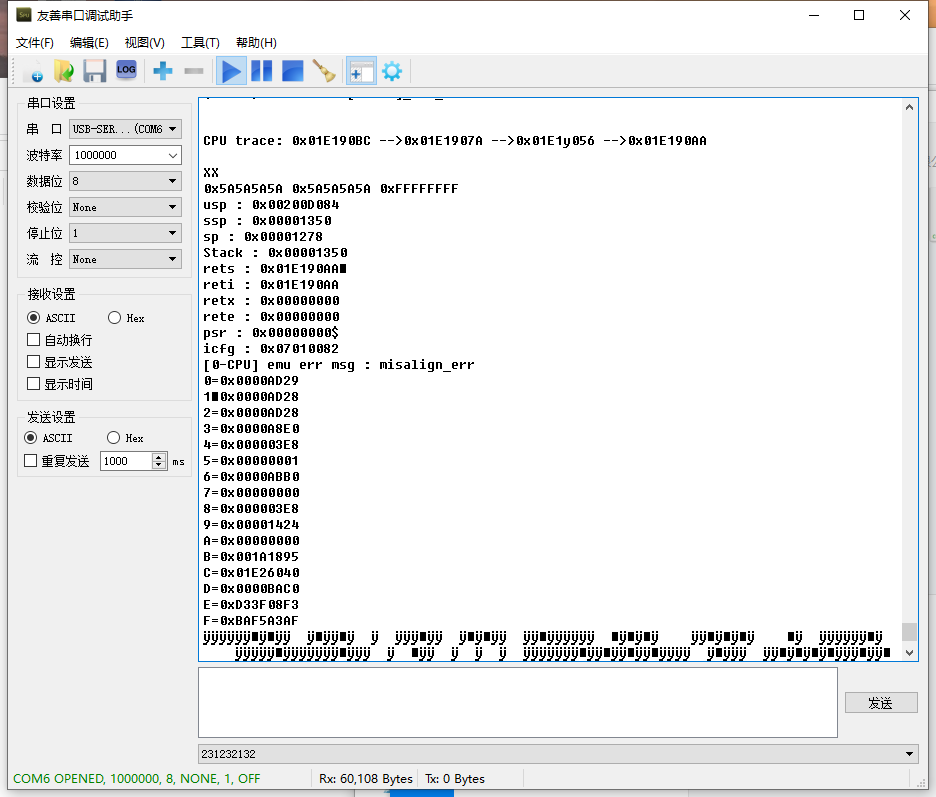
\includegraphics[height=8cm]{rvdd_question.png}
\caption{异常打印}
\label{fig:rvdd_exeception}
\end{figure}
注意:RVDD >= DVDD。

